\documentclass[authordate, empirical,issue]{jote-new-article}

\usepackage{caption}

\usepackage{tabularx}

\usepackage{graphicx}

\usepackage{hyperref}

\usepackage[backend=biber,style=apa]{biblatex}

\addbibresource{bibliography.bib}

\jotetitle{The "function" of art?: challenges of setting up artistic research residencies in elderly care institutions}
\keywordsabstract{artistic research, art residencies, arts and healthcare, co-creation}
\abstracttext{In this article, the authors reflect on the co-creative processes of three artistic research residencies in an elderly care institution in Leiden, The Netherlands. The artists were asked to immerse themselves in the institution for half a year, 2 days a week, to carry out practice-based and experience-driven research. Through artistic methods such as sketching, photographing, or creating mockups, the artists were supposed to reflect on their experiences in the institution, in particular on the relation of the residents to staff, caretakers, and their loved ones at home. These reflections were supposed to lead to final artistic works that offer alternative views on the institution and everything happening in it, from the inside out. 
Two challenges became apparent in these residencies: First, balancing the imaginative and speculative artistic process with the urge to "help", to make a meaningful—however instrumental—contribution to the institution on the other. Second, the urge to use spoken language (i.e. dialogue and discussion) quickly dominated the exchange between artists and participants in the institution and threatened the work with artistic materials, which are often not lingual in nature.
The institution itself and its staff are highly thankful for the fresh and sometimes unexpected/unorthodox views of the artists, but do these more 'systemic' observations actually help the artistic process? And what exactly is the value that the arts and artists have to offer with their practices?}
\runningauthor{Hübner et al.}
\jname{Journal of Trial \& Error}
\jyear{2025}
\paperdoi{10.36850/93a5-4283}
\paperreceived{October 23, 2024}
\author[1]{\mbox{Falk Hübner\orcid{0000-0002-1469-1282}}}
\affil[1]{Fontys Academy of the Arts, Tilburg, the Netherlands}
\corremail{\href{mailto:f.hubner@fontys.nl}{f.hubner@fontys.nl}}
\corraddress{Fontys Academy of the Arts}
\runningauthor{Hübner, Keuning, \& Lucas}
\author[2]{\mbox{Gjilke Keuning\orcid{0009-0003-6222-0420}}}
\affil[2]{HKU University of the Arts, Utrecht, the Netherlands}
\author[1]{\mbox{Marijke Lucas\orcid{0009-0005-3219-3294}}}
\paperaccepted{April 2, 2025}
\paperpublished{June 4, 2025}
\paperpublisheddate{2025-06-04}
\jwebsite{https://journal.trialanderror.org}
\setcounter{page}{24}
\jissue{2}
\jvolume{4}
\jpages{24-36}
\specialissue{Scientific Failure and Uncertainty in the Health Domain}
\articletype{Special Issue - Empirical}

\begin{document}
\begin{frontmatter}
  \maketitle
  \begin{abstract}
    \printabstracttext
  \end{abstract}
\end{frontmatter}


	\section{Introduction}



	In this article, we reflect on the co-creative processes of three artistic research residencies in Topaz, an elderly care institution in Leiden, The Netherlands. This project, called "The Art of Bringing Together" (Dutch original: "De kunst van het samen brengen"), was a collaboration between elderly care institution Topaz in Leiden, HKU University of the Arts Utrecht, and Fontys Academy of the Arts Tilburg. Three artists were asked to immerse themselves in this context for half a year, 2 days a week, in order to carry out practice-based and experience-driven research. Through artistic methods such as sketching, photographing, or creating mockups \footnotemark, the artists were supposed to reflect on their experiences in the institution, in particular on the relation of the residents to staff, caretakers, and their loved ones at home. These reflections should lead to final artistic works that offer alternative, imaginative or speculative views on the institution and what happens in it, from the inside out.

	\footnotetext{ For a more substantial catalogue of artistic methods see Badura et al. (2015). For a conceptual framework of method, research strategy and methodology in artistic research, see Hübner (2024, pp. 31-39).}
	\begin{flushleft}
		\begin{takeHomeMessage}
			We concluded that the residency at the Topaz retirement home was not appropriate for research into residents' relationships with loved ones at home. When artists are offered an open way to connect with the social context, they can find ways that resonate with the underlying needs of older people and loved ones. Artistic interventions and expressions respond to questions in social contexts in powerful, imaginative, speculative, and unexpected ways. We argue that being "functionless" offers an essential value: It allows art and artists in healthcare to actually flourish.
		\end{takeHomeMessage}
	\end{flushleft}
	

	\subsection{Alienation in the process of moving from home to care home}



	The point of departure of the research project was the question \emph{how it is possible to create space for that which makes life worth living}. This question quickly proved too open and too large, needing more specificity. Therefore we refocused the project on the challenges Topaz was grappling with, in particular the period when the residents move from home to care home. Topaz wondered:





	\begin{quote}
		
		How can people who grow older stay focused on what is meaningful for them in life—together with their loved ones, friends and family—despite chronic health-issues?\footnote{ The original question in Dutch was: Hoe kunnen mensen bij het ouder worden zich blijven richten op wat er voor hen toe doet - samen met de mensen die voor hen belangrijk zijn - ondanks chronische gezondheidsuitdagingen?}
	\end{quote}









	Topaz is a care home for elderly people who cannot take care of themselves anymore, in the broadest sense and for a variety of reasons. Staff members at Topaz have observed and experienced how difficult the transition from home to care home is, for the residents themselves as well as for partners, friends, and family. Their homes, most of their belongings, surroundings, routines, and relationships get lost, and relationships that do not get lost tend to change drastically.







	Rather than seeing that existing relationships continue, Topaz observed a process of alienation.\footnote{ Such observations and analyses were shared with the project team and the artists during preparatory conversations and a kick-off meeting (see 'The overall process—Getting started […]').} The institution necessarily takes over most of the care, which can feel ambiguous for close relatives who have offered this care up to the point of moving. They can feel as though they are falling short, because they are no longer able to provide the necessary care. Now that their loved one has moved to a care facility, they find themselves in a very different position and are unsure of what they can and should do. They don't want to be in the way, but they are still concerned and worried about their loved one and still want to spend time with them. In this, they feel dependent on the nurses and care professionals. Due to this sense of dependency, they do not dare to ask everything or be critical.







	The professionals, on the other hand, mainly focus on their relationship with the new resident and often do not know how (or have insufficient time) to deal with the close relatives. They do not want to burden the resident's loved ones, who are often exhausted. They also feel responsible for the quality of care, which they are trained and hired for. It is not self-evident to leave caring tasks to family members, even though they have often done this for a long time. Additionally, doing it themselves is often faster, easier, and thus more efficient than continually coordinating with loved ones about who does what. Small initiatives to facilitate more connection with friends and family only develop slowly, due to existing behavior patterns and time pressure, among other reasons.







	For the people moving to a care facility (the residents), it can be a great loss when relationships vanish or change. This is due to two primary reasons: First, relationships are valuable in themselves; they matter, especially during a significant event such as moving. Second, relationships make various important things possible, such as doing enjoyable activities together. There are things that professionals simply cannot take over, but which are lost in the almost automatic process of "taking over everything." And, finally, for the relational activities that professionals and volunteers can take over, there is an increasing scarcity in the available time to perform these tasks.







	\subsection{"Calling for the arts"—Research question, strategy, and the approach of artistic research residencies}







	By collaborating with the arts, Topaz hoped to create room to find new experiences and alternatives, which might provide alternatives to existing patterns. The initial research question was posed mainly by the care institution and had the following form:






	\begin{quote}
			
		How can we contribute to keeping meaningful relations in and after the period of moving (from home to care institution)?\footnote{Dutch original: Hoe kunnen we zorgen dat waardevolle relaties in en na de verhuisperiode behouden blijven? }
	\end{quote}



	{
	\hyphenpenalty=1500
	\exhyphenpenalty=1500
	

	This question was based on the assumption that such relations (with families, partners, or friends) are valuable in themselves and deserve to be kept intact. How can such relations be continued in a process of reduced self-reliance, either through age or health issues? We chose to approach these questions in and through artistic residencies\footnote{The approach of a residency is closely related to \linebreak (auto-)ethnographic methodologies and action research: The artists spend a substantial part of their time in the care institution, with the residents and staff, and a large part of the creation process takes place there. The artists are thereby enabled to experience this context from within, and thus 'to gain insight by being in the same social space as the subjects of their research' (Madden, 2017, p. 1).} and, within them, processes and activities of artistic co-creation. Three artists spent half a year, 2 days per week, in residence in one of the departments at Topaz, using the period of moving "from home to care home" as a lens to work with. By being present and in contact with several actors (people living there, working there, voluntary staff, families and friends), the artists experienced what happened to the relations of the people who have moved. They used their experiences as inspiration to react by means of (co-)creating artistic work. A co-creative approach means that the activities the artists carry out includes the people this work is about; the artists collaborate with them as co-creators. This also means that the artistic work ideally is not created \emph{for} or \emph{about }the context and people in this context, but \emph{with} them. Such artistic processes are characterized by multisensorial, imaginative, and speculative ways of working, and typically lead to new space to develop emerging ideas, feelings and perspectives. The artists let others participate in their experience. In doing so, this work might be able to create a different, more connective perspective on life and care.While the main actors in this approach were the artists (young graduates from two Dutch art academies: HKU University of the Arts Utrecht and Fontys Academy of the Arts Tilburg\footnote{ HKU en Fontys have curated the participating artists together, in consultation with Topaz. Together the entire team was responsible for matching the artists to the teams at Topaz and their departments.}), there were a number of people involved in facilitating, supervising, and working with them: Project leader "Kleinschalig Zorgen" Eva van Zelm coordinated the project at Topaz and was the first point of contact for the artists during their residence. The artists were further supervised by a team from all three participating institutions: trailblazer Arts, Health, and Society Gjilke Keuning and media artist and pedagogue Erwin Slegers (both HKU),\footnote{ Slegers has also worked in geriatric contexts, has experience as caregiver, and is regularly involved in extracurricular projects. } as well as artist-researcher and professor of Artistic Connective Practices Falk Hübner (Fontys). At Topaz, residents, staff, team leaders, and volunteers were also involved. In the final stage of the residencies, industrial designer Marijke Lucas joined the team as a researcher to provide another perspective to the project. Marijke interviewed the artists extensively after the project was finished (R. Krijgsman, personal communication, November 28, 2023; R. Tavoraite, personal communication, November 29, 2023; M. Pietjouw, January 23, 2024). All three artists have read a draft of this article and provided full consent to use their names and professional identities.


	}

	





	In summary, in this project we were mainly interested in developing new perspectives on the life of the elderly with their loved ones, while and after moving from their home into a care institution. At the same time, we aimed to collect and explore new perspectives on working in and through the arts in the area of healthcare—through the methodological approach of artistic residencies.







	\section{The overall process}



	\subsection{Getting started and arriving at the organization }

	{	
	\hyphenpenalty=1500
	\exhyphenpenalty=1500

	The preparation of the project included \mbox{composing} the core team and supervision structure, making contracts, and formalizing informed consent regarding privacy and data storage. Healthcare staff, residents, and families were informed about the project and were asked for consent to participate.







	Three artists were invited to take part in this project: visual and performance artist Rimanta Tavoraite, designer Mandy Pietjouw, and scenographer and multidisciplinary artist Robin Krijgsman.







	The artists met the organization at a kick-off meeting on location, where Topaz staff introduced them to the different locations and the diversity of residents, such as dementia patients and people with somatic complaints or issues of independence (or the lack thereof). The whole team (including Topaz staff, supervisors, and the artists) visited the locations to get a more concrete and practical impression. Based on this information and the visits, the artists chose three separate locations (in exchange with Topaz), different in size and complexity of care that residents need. Mandy went to work at a location where residents with more advanced forms of dementia live, whilst Robin worked at a location for temporary housing, and Rimanta went to a location with residents with (acquired) physical disabilities. To get to know, and get used to the context, residents, and staff, the artists participated in the work in the various departments: They helped with setting up tables, brought residents to their rooms, took walks with residents outside, or just talked with them. At the same time, this was the start of the creative process, which in total consisted of four stages:





	\begin{enumerate}


		\item Observing, experiencing, and participating,



		\item Generate ideas on the basis of these lived experiences,



		\item Reflection and proposition for a work (in whatever kind or form) that meaningfully contributes to the context,



		\item Public manifestation of the work and sharing of the outcomes.


	\end{enumerate}





	While these four stages had been designed for this particular project, they are based on both earlier artistic research work in relation to healthcare in our own institutions (see Dörr \& Hübner, 2017), as well as loosely related to what Anke Coumans (2020) proposes as the first four of five settings of a "designing attitude" in research projects related to dementia care setting: \emph{anecdotal, observing, situating and in scenario}. The five settings of a "designing attitude" build on Isabelle Stengers' concept of an Ecology of Practices, which aims for "new possibilities for practices to be present or to connect" (Coumans 2020, n.p., our translation).



	The core team came together for collective reflection moments four times during these stages, next to weekly individual coaching moments, both online and on site. The core team and staff of the institution met three times: for the kick-off, a mid-process sharing and reflection session, and the public manifestation.



	}



	\subsection{In-between and final reflections}



	{
	\hyphenpenalty=1500
	\exhyphenpenalty=1500



	The first reflection meeting with the core team, heads of departments, and other interested staff took place after the first few months. In this meeting, the artists shared their experiences and ideas that had emerged up to this point. The session finished with a "Rich A4", a reflective work form developed by the HKU professorship Art and Professionalization. In this work form, participants answer a number of reflective, creative, and associative questions on a piece of paper, including drawing and thinking about a title for one's reflections, for example.







	\begin{figure}
		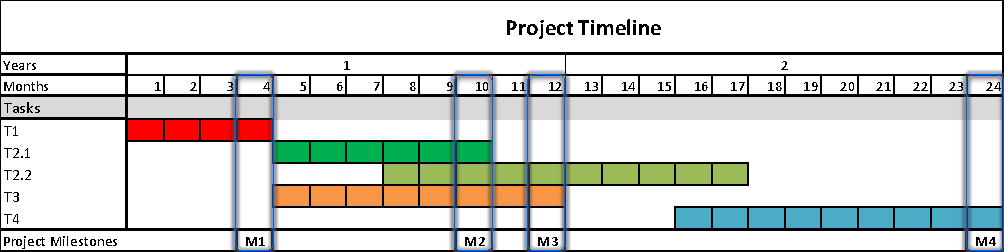
\includegraphics[angle=270, width=\linewidth]{media/fig1.jpeg}

		\caption{A "rich A4", created by one of the participants (anonymized). Image taken by Gjilke Keuning.}



	\end{figure}













	This specific session showed a clear tension and uneasiness. The artists shared their experiences and reflections mainly through telling, using reflective and discursive spoken language (judgmental at times), which resulted in defensive behavior on the side of staff. One of the artists, Rimanta, offered artistic material and a conversation through the metaphor of "Topaz as theater," leading to questions such as: "How does this theater work?" Or: "Which role has the audience in this theater?" This approach proved to be more open and playful and resulted in a much more lively discussion.







	Furthermore, the coaches, artists, and coordinators had three moments of reflection on the project in the form of online sessions. Different forms of reflections were possible. For example, Mandy chose the form of a poem in one of the sessions, a poem she also read during the final presentation.







	\subsection{Final works}







	The final works were presented and shared on one day, organized by and at Topaz in the "living room", a huge space in which residents, families, friends, and staff can come together. Both staff and residents were invited, and the entire team was present, as were the artists. The artists presented their works, which led to several reactions and dialogues. The works were diverse concerning materials, aesthetics, form, or how the works related to the surroundings, people in the institution, how they interacted… All of these parameters were different.







	Mandy's final presentation consisted of two works: A "feel-cloth/-fabric" as a first, smaller study, and a plant made of felt and an inner steel construction as larger work. The plant works in and of itself: Its central idea is to provoke conversations by "standing in the way" and thus bringing residents out of their ordinary rhythm. Residents passed the plant when walking into the living room and were impressed by the craftsmanship, by the soft feel of the plant, or simply by "how beautiful it was."







	\begin{figure}
		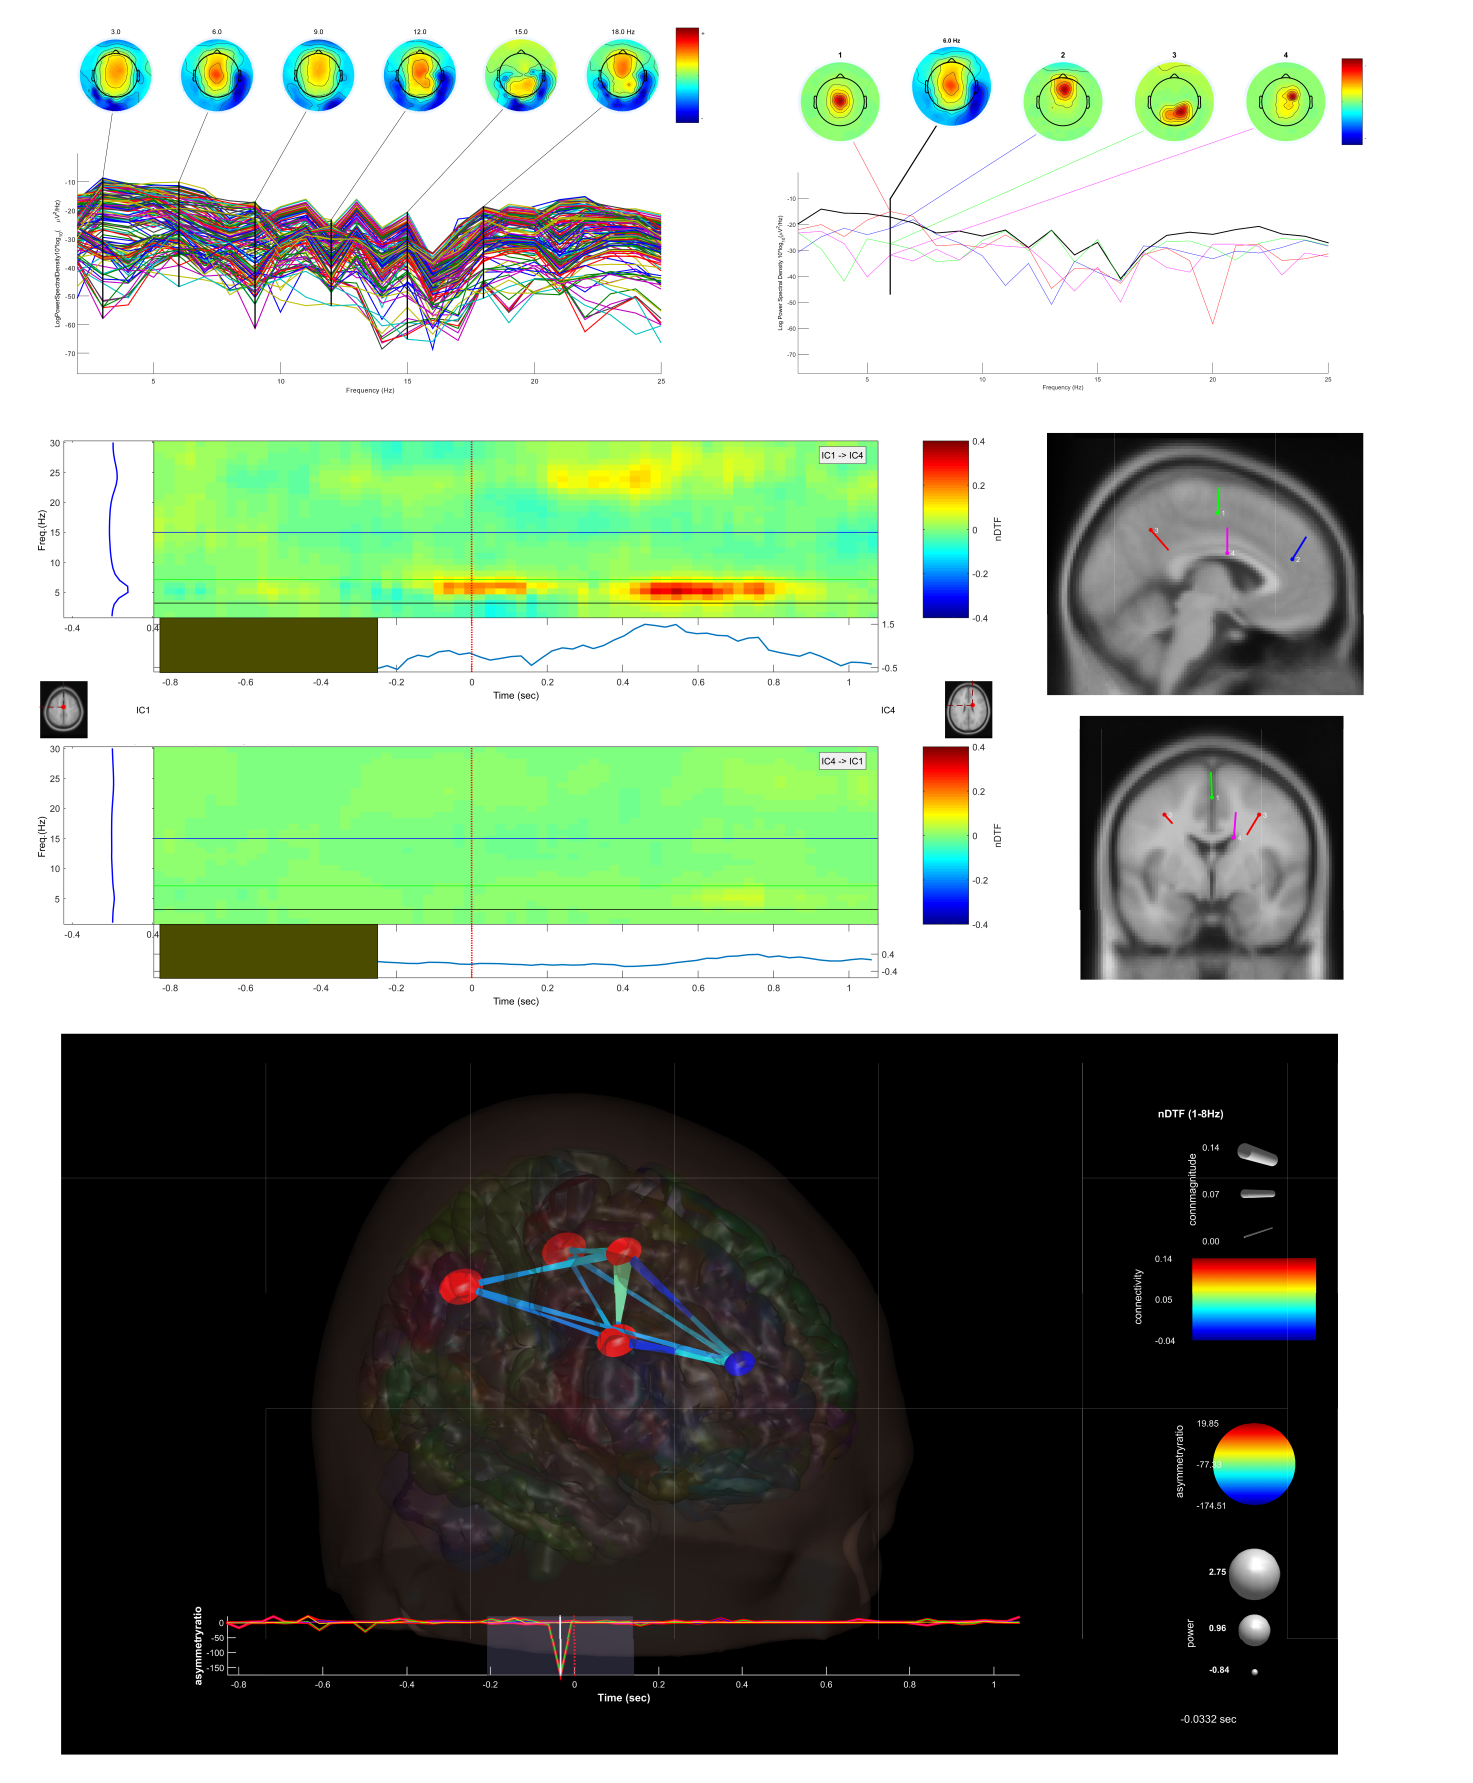
\includegraphics[width=\linewidth]{media/fig2.jpeg}

		\caption{Mandy carries out last adjustments at the plant. Image taken by Gjilke Keuning.}



	\end{figure}









	\begin{figure}
		\includegraphics[width=\linewidth]{media/fig3.jpeg}

		\caption{Mandy's "feel-cloth". Image taken by Gjilke Keuning.}



	\end{figure}













	Conceived as a more general reflection on the healthcare context, Robin's work presented an object in and of itself, as well as a model of an imaginary space. The work reflects on the institution's process of moving into new buildings, and poses the question what happens when furniture is taken away from a place and put into a new place, into a new structure. Which opportunities exist to position things differently, or would one choose for old and familiar structures?







	\begin{figure}
		\includegraphics[width=\linewidth]{media/fig4.jpeg}

		\caption{Robin's model with furniture hanging from the ceiling. Image taken by Gjilke Keuning.}



	\end{figure}












	Rimanta's work, a hybrid between exhibition, performance, and workshop, worked activating for both residents and staff. She used photos of residents as well as her own childhood and combined two photos in one, through a technique of weaving (see Figure 5). The photos sparked memories amongst the older residents in particular and led to engaged conversations, with residents telling stories from their lives. In the interactive part, Rimanta invited the residents and staff to work with various objects themselves, a kind of playful artistic crafting.







	\begin{figure}
		\includegraphics[width=\linewidth]{media/fig5.jpeg}

		\caption{The materials Rimanta offered to work/craft with. See top left for the interwoven photos. Image taken by Gjilke Keuning.}



	\end{figure}








	\begin{figure}
		\includegraphics[width=\linewidth]{media/fig6.jpeg}

		\caption{Two residents in conversation about a photo. Image taken by Gjilke Keuning.}



	\end{figure}







	\begin{figure}
		\includegraphics[width=\linewidth]{media/fig7.jpeg}

		\caption{A resident working with Rimanta's materials. Image taken by Gjilke Keuning.}



	\end{figure}


	}

	\section[Challenges, dillemmas, issues, topics]{Challenges, dilemmas, issues, topics—\protect\\ A catalogue}
	
	
	

	\subsection{General issues/challenges on co-creation}

	{
	\hyphenpenalty=1500
	\exhyphenpenalty=1500

	As in large parts of the healthcare sector, staff regularly changed, worked in different shifts, and on changing days. This presented a general challenge for the artists. There was always a different, new person working in a department and it was difficult to build personal connections. These constant changes made it hard for the artists to explain and clarify what they as artist actually do, how they think and work. It seemed difficult for staff to understand how an artistic process works (and how should they know?), which also resulted in uncertainty regarding mutual expectations.







	The approach of co-creation proved to be a bigger challenge than we expected. In retrospect, none of the three artists has truly worked co-creatively in the sense of involving participants (residents or staff) as partners who more or less create artistic work: Rimanta came closest to this idea, as she built her work by visiting residents and collecting personal stories, experiences, as well as childhood images of residents and staff, and composing new images from them. Mandy, in contrast, "tested out" her ideas and iterations of the work, more comparable to a designer-approach, bringing her designs and iterations into exchange with staff and residents. Robin, instead, appeared to take the position of an outside observer, and took these experiences into his own studio to work. He rather autonomously created—as a comment on this context, so to speak. Concerning the side of the care institution, the staff and residents had no actual reference or frame for artistic practices, which made it a challenge to involve them. We think a guest studio would have been a possible solution for the artists to create their own surrounding within the institution, their own world in which they could invite staff and residents to participate (see the aspect of space below). There are examples of projects in which co-creation with healthcare has worked rather well. For instance, in the project "Onderhuids" (2023--2024), three artists developed art works in co-creation with nurses, in order to reconsider the professional identity of nurses in different nursing contexts, such as community nursing or dementia care departments. Similarly, in "In Search of Stories" (2018--2023), artists worked with terminal cancer patients on co-creating artistic works that reflect on the patients' experiences with the disease, in particular of the diagnosis and how this drastically impacted the understanding of their life stories. However, as these projects held only a loose connection to the healthcare institutions, co-creative processes were naturally much easier to facilitate. Working co-creatively inside of an institution with daily time pressure and high workload on the side of staff remains a challenge.







	In hindsight, it seems to us that the artists a) spent too much time with the first exploratory steps: to "find their place" in the institution, so to speak, to get into meaningful contact and exchange with the people there (including constantly changing staff with different schedules); and b) spent this time observing and holding conversations, largely based on spoken language, rather than immediately translating these experiences into first sketches or small experiments. This resulted in a quite late start of working with and creating artistic materials—a late start of engaging in the (co-)creative and artistic process.







	As a more general issue resulting from the initial design of the project, we observed in the staff an expectation of a functional, instrumental stance or expectation towards the arts,—the arts as a problem-solver—and realized that the artists tended to behave towards caring-for, and easily adopted such an instrumental position. In the next few sections, we have compiled a kind of collection or "catalogue" of issues and challenges that emerged during the process of the residencies—starting with exactly the point of instrumentality and function.




	}


	\subsubsection{Equality and reciprocity as a point of departure—what is the "function" of art?}


	
	{
	\hyphenpenalty=1500
	\exhyphenpenalty=1500



	The project and funding application were initiated by Topaz. This, however unintended, somewhat higher degree of influence (which included posing the initial research question up to the phase of reporting) made it challenging for all parties to find a reciprocal balance: We realized an overall tendency to consider the artistic process and work as "helping healthcare professionals," which in our view limited the actual strength and potential of artistic practice. The artists felt they needed to justify their presence in the departments, instead of fully engaging in an artistic and creative process. They experienced that it was much easier to make connections with the residents than with staff.







	Based on our experience, in this project as well as earlier ones on the intersection of arts and healthcare, we argue for two important points: First, this work would benefit from a more open, equal, and reciprocal relationship between artist, healthcare professional, and patient/resident/participant. Second, the notion of \emph{not knowing}, while challenging, should be granted a much bigger place in all stages, from observing, creating, and reflecting up to the final report. We witnessed a tendency to aim for concrete, directly "usable" output that can be instrumentalized: "Designing a plant is nothing new, what do we gain with this at Topaz?" In our experience, this tendency results in a loss of the actual stories, the moments in which people were truly moved in their emotions or imaginations, and the reflection on the deeper, somewhat hidden, values underlying the research question. Interestingly, we saw that a new space for ideas, emotions, and perspectives arose in situations when artistic material was part of or impulse for starting an exchange, from where a more connective relationship emerged.



	\subsection{The curation of the artists}

	

	This project made very clear that—as expected and as well-known—social contexts are complex and vulnerable, and healthcare contexts are no different. While it was part of the concept and design of the project to invite young artists, alumni from our institutions, in hindsight we should have spent more time thinking about the exact criteria for choice and curation of artists. This includes criteria such as artistic profile, age, and experience.



	While the project was designed as a trajectory including a co-creative artistic approach, it appeared that two of the three artists had insufficient experience with working co-creatively, especially in complex societal contexts. This was not clear enough during the recruitment period. This lack of experience very likely brought them towards "falling back" into the approach of working autonomously in the artist's studio, rather than making their work as much as possible in context, co-creatively. Another aspect is that more experienced artists (more experienced in their own work, in working co-creatively, and with working in social contexts) are typically better able to handle the various, complex parameters of a social context, are more aware of the pitfalls, and can act on them as soon as they appear. In this project, this was delayed, because issues were acknowledged late and supervisors needed to address them. This is no judgement of the three artists participating in this project: The curation was the responsibility of us, the project's core team, and the issue of recruiting young and (in some respects) inexperienced artists was an explicit learning point for us.

	

	

	In earlier, successful projects of transdisciplinary co-creation between arts and healthcare, we observe the crucial difference that artists were more experienced professionals, with both a well-developed co-creative practice, as well as sufficient experience in working transdisciplinary and in complex situations and contexts. An example can be found in the project IYANTWAY (\emph{If you are not here, where are you?}) in which artists worked in co-creation with patients experiencing "absences," a light form of epilepsy (Dörr \& Hübner, 2017). This project at Topaz provided us with a clear indication that this is an aspect that should not be underestimated or overlooked.


	

	\subsection{Was the "assignment" too confusing, unclear, or too open?}



	At several points during the process we observed a certain confusion among the artists. As supervising team, we wondered if the "assignment," or question to the artists, was actually working in the way we envisioned it from the outset. Did we ask the artists to solve anything, or to engage in an open, co-creative process in a societal context? Should the final products lead to a solution, service, or experience that would improve the target group in one way or another? Does it need to be user-friendly? Could it offer alternative, less expected ideas and questions, or would that already be "too much art?" All three artists were confused regarding responses to these questions, and it remained unclear for them what was expected.





	

	The terminology in the project description did not really help to clarify this, as (in the Dutch context, at least) the term "design" typically implies some kind of problem-solving stance. This implication would also suggest more proximity towards the functional use of art, mentioned above. In supervision conversations we instead aimed for a more open artistic exploration, which produced confusion during the artists' day-to-day work in the departments.



	



	In other words, calling our artists "designers" but treating them as artists caused confusion. We are mentioning this explicitly as this seems to be such a small detail (at least it seemed to us), but it had more substantial consequences than we expected. While we as supervisors and creators of the project might not make such a huge difference between the two terms (or at least understand the "designer-artist"-pair as a flexible relationship in which many hybrid positionalities are possible), others might actually differentiate them, including the artists in residence themselves.







	A second point of confusion lay in the initial setup of the project and research question. The artists were asked to look at meaningful relations of the residents before moving to the care institution and how these relationships could be kept intact. However, virtually all of the work happened within the walls of Topaz, while contact with family and friends remained difficult. For residents, the period before moving was already quite far away for them, and questions about this were unproductive. It might have been advisable to change the research question towards what makes life meaningful \emph{in this moment}, without referring to earlier relations too explicitly. Another possibility might have been to include families and friends much more actively from the outset and the design phase, to ensure participation.







	Next to this confusion, we wonder if the process we designed worked for the artists. We offered the four stages to them that we mentioned above under "Getting started." However, the artists experienced this approach and process as being too open—and thus as too vague or unclear. This might be one of the reasons they started quite late with creating actual artistic material—an aspect that will come back later in the section "On (too much) reflection through language." This issue also has a direct relationship to what we described in the previous section on curation: While the younger, less experienced artists of our project experienced this process as too open, artists with more experience in this kind of work may have had no issue with openness. For them, it might have provided a more immediate way of working with their own approach, without waiting for clarifying instructions.







	\subsection{Balance between the artistic and the urge to help}







	We clearly experienced the challenge to balance the more imaginative and associative artistic process on the one hand, and the urge to "help," to make a meaningful (and instrumental) contribution to what happens in the institution on the other. The initial idea was that the artists would get to know the atmosphere, dynamics, and rhythm of the departments by helping in the day-to-day routine, and that this would also help them to get into contact with staff and residents. For some of the artists, this was natural to do, while for others this was less the case. However, all artists felt some kind of pressure to help their department, which took time and attention away from their artistic process. In hindsight, we analyze that the time for observing and helping and the time for the artistic process were not balanced; one could argue that the approach "mispositioned" the artists in the departments, exactly because they were immediately instrumentalized.







	For the artists, it could be hard to differentiate between personal engagement and the role of a professional. The boundary between the two is personal and different for everyone, and not every artist is willing to step into such a helping role. Especially for the young artists in this project, it proved difficult to guard this boundary.







	All three artists were struggling with this "task to help" and its effect on their function and professional identity as artists. Additionally, they felt little space to inquire what actually would have been an appropriate way to interpret "helping" in service of the artistic process. Our analysis is that, as core team of the project, we could or should have spent more time to communicate this particular tension with the organization and staff, in order to create space for the artists to explore this.



	\subsection{A lack of artistic and safe space}



	The project showed us how important it is to create a safe space (both physically and mentally) in which artistic processes and dialogues can come to fruition—for everyone involved. Neither us, nor Topaz considered a place such as a studio or other kind of dedicated physical space in which the artists could work. Nor was there any space available for artists to leave materials or objects behind, which posed logistical challenges. Every activity needed to happen surrounded by staff and residents. This led the artists to feel insufficiently free to experiment with materials and methods and hindered them to "step out" of the daily dynamics of the care institution. As soon as they were on site, it was virtually impossible to take more distance and time to think and reflect on their observations. This led to an experienced lack of mental space as well. The artists experienced it as challenging that they repeatedly had to explain that creating artistic work inevitably needs to include preparatory work and research. They felt cramped and de-focused being asked time and time again if they had already "made" anything. In hindsight, a simple space with a door that could be closed would have been a relatively easy solution to help focusing, and to create a sort of "in-between-space", a space safe enough to be a brave space (Cairo et al., 2021, pp. 197-201), into which the artists could invite staff and residents for more artistically-focused explorations and conversations. The artists could have used such a space as their "own world" into which they could invite others and share their artistic process and thinking, on their own ground, so to speak. At the same time, such a space would have brought our concept of a socially engaged residency in a healthcare context closer to the traditional residency form, which offers artists explicitly the space and time to create, without the concern for unhelpful distractions.







	\subsection{Misguided approach? On (too much) reflection through language}



	Looking at the overall structure of the process in time, we come to two crucial insights: First, the artists spent a considerable amount of time experiencing Topaz through observation and participation, rather than through creating and making sense of it through artistic creation or experiments. Second, the exchange between artists and the actors in the institution was largely dominated by spoken language, rather than through artistic materials (which are often \emph{not} lingual in nature). And while the institution's staff members were typically highly thankful for the fresh and sometimes unexpected or unorthodox views of the artists, we observed that this exchange through language also had the potential to lead to judgments and unnecessary "tips" towards the institution, which in turn led to defensive behavior of the staff and unhelpful tensions especially between artists and staff. On the other hand, in moments when an artist shared artistic material, sketches, or creative assignments or exercises, the conversation took a much more exploratory, associative, and fruitful direction, where a true, non-judgmental exchange of ideas took place.







	We argue that it is (or actually it should be) exactly the more open, speculative, and creative nature of artistic work and practice that creates a less judgmental and more meaningful dialogue and connection between the arts and institutional healthcare. Artistic materials also have more means and potential to make radical propositions and speculate with them. Statements or thoughts such as "It is only natural that the elderly in such institutions are not happy, as no one asks them what they want\footnote{This quote is a statement, or rather provocation, uttered by one of the artists during an in-between reflection session with the core team and staff from Topaz.}" sound unqualified and blunt when spoken, but (after discussion and gaining nuance) can turn into powerful incentives for making artistic work. In turn, this work can facilitate a richer, more empathetic, reciprocal, and impactful dialogue. Taking this further, it is exactly the open, exploratory, and speculative nature of artistic work that can facilitate connectivity, rather than dialogue through spoken language \emph{per se}. It is clear that we have only been able to see this in hindsight, but did not realize the nature of the conversations as being too much focused on language in time. Or—to be more precise—we recognized this, but were unable to change the nature of the conversations accordingly.







	An important lesson that has been mentioned a few times already: It is crucial in such residencies that artists start by making, creating material, trying out—just starting, in fact—much earlier, or even as early as possible. This has two important consequences, on the level of documenting experiences and insights, and on the level of reporting.







	\subsubsection{On documenting:}







	There have been a number of valuable dialogues and encounters between the artists and especially staff members, but we have not been able to document these in a way that is experienceable in other means than written language. To provide an example: In some cases the artists experienced being intensely emotional or sad when they witnessed how the elderly people were not allowed to make specific decisions themselves anymore. While this can be captured in words to some extent (which the artists did, in the form of notes, bullet points or quotes), reading these notes feels pale or shallow compared to the actual experience; it is difficult to understand the true impact and essence of these experiences. If the artists would have been able to capture this in the form of artistic materials (drawings, animations, sounds), this would likely have had the potential to offer a more experiential, deeper and richer way of sharing these experiences.







	\subsubsection{On losing insights and nuances in reporting:}







	This loss of the quality and nature of the experience directly translates to the final documentation and report of the residencies and the project as a whole. The report has been written by Topaz, the healthcare institution, exclusively in text. The "artistic qualities" (in observations and experiences, concerning ethical, societal or political insights) were almost entirely lost, due to the sole focus on written language and the absence of artistic materials. While the potential of such a project lies in the possibility to come to new insights in healthcare through artistic processes and works, leaving exactly those modes of artistic practice out of a report inevitably results in a loss of this potential—and the imagined and ambitioned innovation in healthcare.




	}


	\section{Final reflections}
	\begin{originalPurpose}
		The aim of the collaboration between Topaz and the three artists was to develop new perspectives on the lives of the elderly with their loved ones during and after the move from their home to a care institution. At the same time, we wanted to collect and explore new perspectives on co-creative working in and through the arts in the field of healthcare—through the methodological approach of artistic residencies. We wanted to research the position of the artists in the context and at the same time learn about their artistic skills and talent. Taking this further, we were curious if the open, exploratory, and speculative nature of artistic work was able to facilitate connectivity better than dialogue through spoken language. To create free space for this we wanted to prevent the artists from being positioned or seen as an instrumental "problem solver" in the department, which could limit their artistic freedom. Finally, we were curious about the working or not-working elements of this crossover practice.
	\end{originalPurpose}



	{
	\hyphenpenalty=1500
	\exhyphenpenalty=1500

	There are a few aspects that seem helpful to us to be reminded of when it comes to artistic research residencies in healthcare institutions. Obviously, a number of issues and challenges described in the previous sections are entangled: For example, the fact that the artists, being less experienced in co-creation \emph{in situ}, fell back into working in their studio, likely could have been mitigated to some degree (or potentially solved) by having a dedicated space for them in the institution. In summary, we propose a set of five recommendations, which are elaborated on further below:





	\begin{enumerate}


		\item Take sufficient, probably more time than one estimates necessary, to carefully design such a transdisciplinary project, and consider which kinds of preparation everyone needs,



		\item
		Allow artists to take a position of being "function-less" and practice to see this as a meaningful value,



		\item Design this "function-less-ness" specifically into a project in the form of time and space for the artistic-creative process,



		\item
		Make sure that artists start working with their respective media and disciplines, and making artistic materials, as early in the process as possible,



		\item If possible, provide some kind of dedicated studio space for artists to work in and develop (unfinished) material.


	\end{enumerate}





	We have learned that taking (even more) time to design such a project carefully is a key factor. This includes the complex task of clarifying and negotiating the expectations for all participating actors: the care institution, its staff, residents, potentially loved ones, artists, and supervising research institutions. These are all participating voices that need a certain amount of synchronization (see Christophe, 2017). This synchronization also requires careful consideration of the relationship between a healthcare institution's question and the approach with which the project will be conducted in and through artistic practice.







	If there is one underlying red thread in the challenges we describe, it is the question of what function artists can have in a context of healthcare. Or, more provocatively: In which way can \emph{artists be allowed to be function-less}? Everyone in a healthcare context has a function, including residents, patients, friends, and family. In their best moments, the artists in our residencies experienced themselves as the only ones who are "free of function" (R. Krijgsman, personal communication, November 28, 2023). Resonating with this, Mandy reported being asked: "What are you actually doing here?" We argue that this notion of being "without function" or being "functionless" offers an essential value: to let the arts and artists in healthcare contexts actually come to fruition—which, at the same time, can be confronting and feel risky for healthcare staff, as it works to much against notions of efficiency, clear task-division, and scheduling, which are so ubiquitous in this field. Understandably, being functionless provokes initial reactions that there won't be any (positive) impact or change. However, we argue that, in potential, the exact opposite is the case: It is exactly by facilitating artists with an open environment to connect to a social context that they can find ways that resonate with the underlying questions and issues of this context and develop works, interventions, and artistic utterances that react in a powerful, imaginative, and speculative way to this context—in ways that one could never expect by giving a more or less exact or concrete assignment.







	Our recommendation is thus to spend more time thinking about, and designing this function-less-ness\footnote{ Obviously, this is more than just a "negative" argument: Artists can open up, reflect on experiences and issues they encounter, and thus put these "on the agenda", which is not literally without function, but not being "in service" either.} into such projects from the outset: to provide more emotional-creative capacity for making, more openness for artists to create and react to what they experience in the context (of a care institution, in this case), and, by this, enable artists to think through their practice—to think through art (Hübner, 2022, p. 8). This is considerably different from the more romantic notions of independency, "autonomous art" or "artistic freedom;" we argue for an open sense of situated relationality, where artists can productively relate in a meaningful way, while not being instrumentalized.







	Following up on this point, this means that artistic and research practice need to take a much more prominent place, both in terms of literally creating artistic materials, as well as documenting and reflecting along the way. We argue that artists should aim for working with their own media (objects, color, sound, still and moving images, sketches, drawings, and so on) as early as possible. This does not mean they need to create artistic \emph{works} immediately, but rather observe, document, and reflect on a given social context by means of artistic media, which in turn will lead to a less forced but more natural way of creating actual works.







	Finally, and again emerging from the previous point, we will reiterate the need for a physical space for artists in such residencies. As mentioned before, a physical space can enhance a clear positioning of artists in an organization, and it can provide them with a "temporary home," both for themselves and for how staff experiences them. A (temporary) studio can be a space to be able to work, where materials can stay, lie around, where artists can play with ideas without having to justify them at any given moment (which can feel unsafe)—and a place to invite staff and residents into. A space safe enough to be brave, and thus a space to make it possible to be an artist in healthcare; not in literal service, not as a therapist, not "in function," but as an artist.

	}


	\section{References}

	{
	\hyphenpenalty=10000
	\exhyphenpenalty=10000

	Badura, J., Dubach, S., Haarmann, A., Mersh, D., Rey, A., Schenker, C., \& Toro Pérez, G. (2015). \emph{Künstlerische Forschung: Ein Handbuch}. Diaphanes.







	Cairo, A., Misiedjan, D., \& van Uden, J. (2021). \emph{Holding space. A storytelling approach to trampling diversity and inclusion}. Aminata Cairo Consultancy.







	Christophe, N. (2017). The art is in the encounter. In H. Dörr \& F. Hübner (Eds.), \emph{If you are not there, where are you?} (pp. 88-105). International Theatre \& Film Books Publishers.







	Coumans, A. (2020). Ontwerpen in het hier en nu. De artistieke attitude in de zorg voor mensen met dementie. \emph{Forum+,} \emph{27}(2), 3-13. \url{https://doi.org/10.5117/FORUM2020.2.002.COUM}







	Dörr H., \& Hübner, F. (Eds.) (2017). \emph{If you are not there, where are you?} International Theatre \& Film Books Publishers.







	Hübner, F. (2022, November 18). \emph{In good company. Think we must}. Fontys Fine and Performing Arts. \url{https://www.researchcatalogue.net/view/2606237/2606238}







	Hübner, F. (2024). \emph{Method, methodology and research strategy in artistic research. Between solid routes and emergent pathways}. Routledge.







	Madden, R. (2017). \emph{Being ethnographic: A guide to the theory and practice of ethnography}. SAGE Publications Ltd. \url{https://doi.org/10.4135/9781529716689}

	}




\end{document}